\documentclass[11pt]{article}
\newcommand{\MODULETAG}{Module 4\,\textbar\,Variography}
% ===== Toro Resource Estimation Course - shared PDF preamble =====
\usepackage[a4paper,margin=2.4cm,headsep=14pt]{geometry}
\usepackage{amsmath,amssymb}
\usepackage{lmodern}
\usepackage[T1]{fontenc}
\usepackage[utf8]{inputenc}
\usepackage{microtype}
\usepackage{graphicx}
\usepackage{booktabs}
\usepackage{array}
\usepackage{enumitem}
\usepackage{xcolor}
\usepackage{titlesec}
\usepackage{fancyhdr}
\usepackage[most]{tcolorbox}
\usepackage{listings}
\usepackage{caption}
\usepackage[hidelinks]{hyperref}

% ---- palette ----
\definecolor{navy}{HTML}{1F2A44}
\definecolor{navy2}{HTML}{2B3A5C}
\definecolor{bronze}{HTML}{C8702D}
\definecolor{bronzed}{HTML}{A85A1F}
\definecolor{teal}{HTML}{2A7D8C}
\definecolor{tealw}{HTML}{ECF4F5}
\definecolor{ink}{HTML}{26303F}
\definecolor{paper2}{HTML}{F3EDE1}
\definecolor{line}{HTML}{D8D4CB}
\definecolor{codebg}{HTML}{1C2433}
\definecolor{good}{HTML}{3F7D5A}
\definecolor{warn}{HTML}{B4451F}

\color{ink}
\setlength{\parindent}{0pt}
\setlength{\parskip}{6pt}
\linespread{1.06}

% ---- section styling ----
\titleformat{\section}{\Large\bfseries\color{navy}}{\thesection}{0.6em}{}
\titleformat{\subsection}{\large\bfseries\color{navy2}}{\thesubsection}{0.6em}{}
\titleformat{\subsubsection}{\normalsize\bfseries\color{bronzed}}{}{0em}{}
\titlespacing{\section}{0pt}{16pt}{6pt}
\titlespacing{\subsection}{0pt}{12pt}{4pt}

% ---- header / footer ----
\pagestyle{fancy}
\fancyhf{}
\renewcommand{\headrulewidth}{0.4pt}
\renewcommand{\footrulewidth}{0pt}
\fancyhead[L]{\footnotesize\color{navy2}\MODULETAG}
\fancyhead[R]{\footnotesize\color{navy2}Toro Tin Project\,\textbar\,ANRML26-137}
\fancyfoot[C]{\footnotesize\color{navy2}\thepage}

% ---- callout boxes ----
\newtcolorbox{keybox}[1][Key concept]{breakable,enhanced,
  colback=paper2,colframe=bronze,boxrule=0pt,leftrule=4pt,
  arc=2pt,left=10pt,right=10pt,top=8pt,bottom=8pt,
  fonttitle=\bfseries\sffamily\small\color{bronzed},title={#1}}
\newtcolorbox{torobox}[1][Toro application]{breakable,enhanced,
  colback=navy!6,colframe=navy,boxrule=0pt,leftrule=4pt,
  arc=2pt,left=10pt,right=10pt,top=8pt,bottom=8pt,
  fonttitle=\bfseries\sffamily\small\color{navy},title={#1}}
\newtcolorbox{pitbox}[1][Common pitfall]{breakable,enhanced,
  colback=warn!7,colframe=warn,boxrule=0pt,leftrule=4pt,
  arc=2pt,left=10pt,right=10pt,top=8pt,bottom=8pt,
  fonttitle=\bfseries\sffamily\small\color{warn},title={#1}}
\newtcolorbox{notebox}[1][Note]{breakable,enhanced,
  colback=tealw,colframe=teal,boxrule=0pt,leftrule=4pt,
  arc=2pt,left=10pt,right=10pt,top=8pt,bottom=8pt,
  fonttitle=\bfseries\sffamily\small\color{teal},title={#1}}
\newtcolorbox{defbox}[1][Definition]{breakable,enhanced,
  colback=good!7,colframe=good,boxrule=0pt,leftrule=4pt,
  arc=2pt,left=10pt,right=10pt,top=8pt,bottom=8pt,
  fonttitle=\bfseries\sffamily\small\color{good},title={#1}}
\newtcolorbox{objbox}{enhanced,colback=navy,colframe=navy,
  arc=3pt,left=12pt,right=12pt,top=10pt,bottom=10pt,
  coltext=white}

% ---- python code ----
\lstdefinestyle{py}{language=Python,
  basicstyle=\footnotesize\ttfamily\color{white},
  keywordstyle=\color{bronze},commentstyle=\color{line},
  stringstyle=\color{teal!60!white},backgroundcolor=\color{codebg},
  numberstyle=\tiny\color{line},showstringspaces=false,
  breaklines=true,frame=single,framerule=0pt,
  rulecolor=\color{codebg},xleftmargin=8pt,xrightmargin=4pt,
  aboveskip=10pt,belowskip=6pt,framexleftmargin=8pt,
  framexrightmargin=8pt,framextopmargin=6pt,framexbottommargin=6pt}
\lstset{style=py}

% ---- equation box ----
\newtcolorbox{eqbox}{enhanced,colback=white,colframe=line,
  boxrule=0.6pt,arc=2pt,left=8pt,right=8pt,top=4pt,bottom=4pt,
  before skip=10pt,after skip=10pt}

% ---- captions ----
\captionsetup{font={small,it},labelfont={bf,color=navy},labelsep=endash}

% ---- module title macro ----
\newcommand{\moduletitle}[3]{%
  {\sffamily\bfseries\footnotesize\color{bronze}\MakeUppercase{#1}\par}
  \vspace{2pt}
  {\sffamily\bfseries\LARGE\color{navy}#2\par}
  \vspace{3pt}
  {\small\itshape\color{navy2}#3\par}
  \vspace{4pt}{\color{line}\hrule height 1.5pt}\vspace{12pt}}

\begin{document}

\moduletitle{Module 4 of 6}{Spatial Continuity and Variography}{The
heart of geostatistics: measuring, modelling and exploiting spatial
dependence in grade}

Classical statistics treats samples as independent --- but grade samples
are not independent: two pits 50 m apart tell you more about each other
than two pits 5 km apart. Variography is the mathematics that measures,
models and exploits that spatial dependence. Every estimate in Module 5
is built on the variogram fitted here.

\begin{objbox}
{\sffamily\bfseries\color{bronze}LEARNING OBJECTIVES}
\begin{itemize}[leftmargin=14pt,itemsep=2pt]
\item Explain the regionalised variable and the random function model.
\item State the second-order and intrinsic stationarity hypotheses.
\item Define the covariance and the semivariogram and derive the
relationship between them.
\item Compute an experimental variogram and read its nugget, sill and
range.
\item Fit a licit variogram model and recognise anisotropy.
\item Build and interpret the Toro SnO$_2$ variogram.
\end{itemize}
\end{objbox}

\section{The regionalised variable and the random function}

Grade is a number attached to a location, written $z(\mathbf{x})$.
Matheron called such a quantity a \textbf{regionalised variable} ---
distributed in space with a \emph{structured} character (reflecting
geology) and a \emph{random} character (point-to-point fluctuation no
deterministic equation predicts).

We have exactly one grade value at each sampled point --- one realisation
of reality. To speak of probability and variance we model that single
reality as a \textbf{random function}: at every location $\mathbf{x}$,
treat the grade $Z(\mathbf{x})$ as a random variable; the whole collection
is a random function. Our measured map is one realisation drawn from an
imagined ensemble of geologically possible deposits.

\section{Stationarity hypotheses}

We have one realisation but need ensemble averages. Stationarity is the
bridge: it lets us replace ensemble averages with spatial averages over
our single dataset.

\textbf{Second-order (weak) stationarity} requires a constant mean and a
covariance depending only on the separation vector $\mathbf{h}$:

\begin{eqbox}
\[ \mathbb{E}[Z(\mathbf{x})] = m, \qquad
   \operatorname{Cov}\!\big[Z(\mathbf{x}),Z(\mathbf{x}+\mathbf{h})\big]
   = C(\mathbf{h}) \tag{4.1--4.2}\]
\end{eqbox}

Setting $\mathbf{h}=0$ gives $C(0) = \operatorname{Var}[Z(\mathbf{x})]$,
the variance of the random function. Second-order stationarity requires
a finite $C(0)$. Some geological variables have variance that grows
without limit as the domain expands, and for them geostatistics relies on
a weaker assumption.

\begin{keybox}[The intrinsic hypothesis]
The intrinsic hypothesis requires stationarity only of the
\emph{increments} $Z(\mathbf{x}+\mathbf{h})-Z(\mathbf{x})$:
\[ \mathbb{E}\!\big[Z(\mathbf{x}+\mathbf{h})-Z(\mathbf{x})\big]=0,
   \quad
   \operatorname{Var}\!\big[Z(\mathbf{x}+\mathbf{h})-Z(\mathbf{x})\big]
   = 2\gamma(\mathbf{h}) \]
Every second-order stationary function is intrinsic but not the reverse.
This is the working assumption of practical geostatistics.
\end{keybox}

\section{The semivariogram and its link to covariance}

The \textbf{semivariogram} $\gamma(\mathbf{h})$ is the central tool of
geostatistics --- half the variance of the increment:

\begin{eqbox}
\[ \gamma(\mathbf{h}) = \tfrac{1}{2}\operatorname{Var}\!\big[
   Z(\mathbf{x}+\mathbf{h})-Z(\mathbf{x})\big]
   = \tfrac{1}{2}\,\mathbb{E}\!\Big[\big(Z(\mathbf{x}+\mathbf{h})
   -Z(\mathbf{x})\big)^2\Big] \tag{4.3--4.4}\]
\end{eqbox}

Small $\gamma$ means values stay alike across $\mathbf{h}$; large $\gamma$
means they decorrelate.

\begin{notebox}[Derivation: $\gamma(\mathbf{h}) = C(0) - C(\mathbf{h})$]
Expanding the square in (4.4):
\[ 2\gamma(\mathbf{h})=\mathbb{E}[Z(\mathbf{x}+\mathbf{h})^2]
   +\mathbb{E}[Z(\mathbf{x})^2]
   -2\mathbb{E}[Z(\mathbf{x}+\mathbf{h})Z(\mathbf{x})] \]
For any random variable, $\mathbb{E}[Z^2]=C(0)+m^2$. And
$\mathbb{E}[Z(\mathbf{x}+\mathbf{h})Z(\mathbf{x})]=C(\mathbf{h})+m^2$.
Substituting:
\[ 2\gamma(\mathbf{h}) = 2C(0)+2m^2-2C(\mathbf{h})-2m^2
   = 2\big(C(0)-C(\mathbf{h})\big) \]
\[ \boxed{\;\gamma(\mathbf{h})\;=\;C(0)-C(\mathbf{h})\;} \]
\end{notebox}

At $\mathbf{h}=0$, $\gamma=0$: a value is identical to itself. As
$\mathbf{h}$ grows, $C(\mathbf{h})$ decays towards zero, so $\gamma$
\emph{rises} towards $C(0)$, the variance. The variogram is the
covariance turned upside down.

\section{The experimental variogram}

From data we estimate (4.4) with the Matheron estimator:

\begin{eqbox}
\[ \hat{\gamma}(\mathbf{h}) = \frac{1}{2\,N(\mathbf{h})}
   \sum_{i=1}^{N(\mathbf{h})}
   \big[z(\mathbf{x}_i)-z(\mathbf{x}_i+\mathbf{h})\big]^2 \tag{4.5}\]
\end{eqbox}

Real samples are never separated by exactly $\mathbf{h}$, so pairs are
collected into \textbf{lag bins} defined by a lag and a tolerance. Three
rules: each lag should carry at least about 30 pairs (below 20 is noise);
interpret only out to about half the field extent; the lag spacing should
be near the typical data spacing.

\section{Anatomy of the variogram}

A typical variogram rises and flattens. Three parameters describe it.

\textbf{Nugget} $C_0$ --- the apparent jump at vanishingly small $h$.
$\gamma(0)=0$ in theory; a positive intercept means two samples nearly at
the same place still differ. It is micro-scale geological variability
plus Module 2's sampling-and-assay error. Pure unstructured noise.

\textbf{Sill} $C_0+C$ --- the plateau. Under the boxed result of section
4.3 the sill equals the variance $C(0)$ of the data. $C$ alone is the
structured part of the variance.

\textbf{Range} $a$ --- the lag at which the variogram reaches the sill;
the distance of influence. Beyond the range, two samples are
statistically independent.

The most diagnostic single number is the \textbf{relative nugget}:

\begin{eqbox}
\[ \text{relative nugget} = \frac{C_0}{C_0+C} \tag{4.6}\]
\end{eqbox}

Below 0.25: well-structured. 0.25--0.5: moderate noise. Above 0.5: highly
erratic --- half the variability is unstructured.

\section{Variogram models}

The experimental variogram is known only at noisy, discrete lags. Kriging
needs $\gamma(\mathbf{h})$ everywhere --- and the function must be
\textbf{conditionally negative semi-definite} so the kriging system has a
unique solution and never returns negative variance. So we fit one of a
small library of \emph{licit} models.

\subsection*{Spherical --- the workhorse}
\begin{eqbox}
\[ \gamma(h)=\begin{cases}
   C_0+C\!\left[\dfrac{3h}{2a}-\dfrac{1}{2}\!\left(\dfrac{h}{a}\right)^{\!3}
   \right], & 0<h\le a\\[2mm]
   C_0+C, & h>a \end{cases} \tag{4.7}\]
\end{eqbox}
Reaches the sill exactly at the range $a$, linear near the origin. Used
for the Toro estimate.

\subsection*{Exponential}
\begin{eqbox}
\[ \gamma(h)=C_0+C\left[1-\exp\!\left(-\tfrac{3h}{a}\right)\right]
   \tag{4.8}\]
\end{eqbox}
Approaches the sill asymptotically; $a$ is the practical range where 95\%
of the sill is reached. Suits erratic mineralisation.

\subsection*{Gaussian}
\begin{eqbox}
\[ \gamma(h)=C_0+C\left[1-\exp\!\left(-\tfrac{3h^{2}}{a^{2}}\right)
   \right] \tag{4.9}\]
\end{eqbox}
Parabolic at the origin: describes extremely continuous properties
(thicknesses, weathering surfaces). Use with care --- numerically
unstable without a nugget.

\subsection*{Power --- unbounded}
\begin{eqbox}
\[ \gamma(h)=C_0+p\,h^{\,\omega},\qquad 0<\omega<2 \tag{4.10}\]
\end{eqbox}
No sill, no range. Describes a variable that decorrelates without limit.

A sum of licit models is itself licit. Real deposits often need a
\textbf{nested} variogram --- a nugget plus a short-range structure
(local mineralisation) plus a long-range structure (regional trend).

\section{Anisotropy}

Grade continuity is rarely the same in every direction. A placer is more
continuous \emph{along} its palaeochannel than across it. Variograms are
computed \textbf{directionally} --- pairs binned not only by distance
but by the azimuth of the vector joining them, within an angular
tolerance.

When directional variograms share a sill but differ in range, the
structure has \textbf{geometric anisotropy}, described by an ellipse
(major axis along the direction of greatest continuity). When the sill
itself changes with direction, it is \textbf{zonal anisotropy}. A
\textbf{variogram map} computes $\hat\gamma$ over a 2D grid of lag
vectors; its elliptical contours reveal both strength and orientation of
anisotropy at a glance.

\section{The Toro variogram, built and fitted}

The variogram is computed on the 26 composited Toro pit grades, with a
180 m lag matching the typical Bishiwai pit spacing. Fitting follows three
defensible decisions: only the six lags carrying at least 20 pairs drive
the fit (the three sparse outer lags are noise); the sill is fixed to the
sample variance (the boxed result of section 4.3); and an isotropic
spherical model is adopted because the directional data cannot resolve
anisotropy.

\begin{figure}[h]\centering
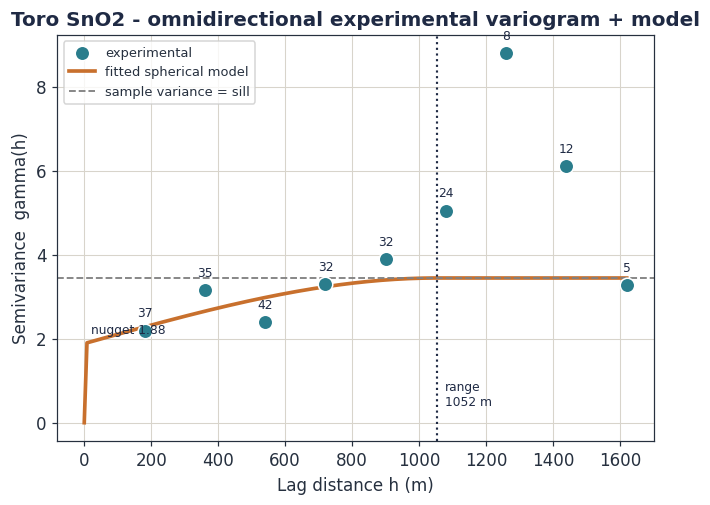
\includegraphics[width=0.78\textwidth]{../assets/figures/fig_variogram_omni.png}
\caption{Toro SnO$_2$ omnidirectional experimental variogram with fitted
spherical model. Pair counts beside each point.}
\end{figure}

\begin{torobox}[The fitted Toro model]
\begin{center}\small
\begin{tabular}{@{}lrl@{}}
\toprule
\textbf{Parameter} & \textbf{Value} & \textbf{Interpretation}\\
\midrule
Nugget $C_0$ & 1.88 & unstructured noise --- sampling + micro-variability\\
Sill $C_0+C$ & 3.44 & total variance of composited grades\\
Range $a$ & 1052 m & distance of grade influence\\
Relative nugget & 0.55 & more than half the variance is unstructured\\
\bottomrule
\end{tabular}
\end{center}
A relative nugget of 0.55 means over half the grade variance has no
spatial structure the data can resolve. Some is the genuine erratic
character of coarse cassiterite; much is the fundamental sampling error
of panned-concentrate sampling. The structured range of about 1 km is
encouraging --- drainage-scale continuity --- but a high-nugget variogram
is a quantitative warning: this data will estimate weakly. Lowering the
nugget is a sampling problem (Module 2), not an estimation problem.
\end{torobox}

\begin{lstlisting}
import numpy as np

def experimental_variogram(x, y, z, lag, nlags, tol=None):
    """Matheron estimator - equation (4.5)."""
    if tol is None: tol = lag / 2.0
    n = len(z)
    dx = x[:, None] - x[None, :]
    dy = y[:, None] - y[None, :]
    h  = np.sqrt(dx**2 + dy**2)
    diff2 = (z[:, None] - z[None, :])**2
    iu = np.triu_indices(n, k=1)
    h, diff2 = h[iu], diff2[iu]
    out = []
    for k in range(1, nlags + 1):
        centre = k * lag
        m = np.abs(h - centre) <= tol
        if m.sum() >= 2:
            out.append((centre, 0.5 * diff2[m].mean(), int(m.sum())))
    return out

def spherical(h, nugget, sill, rng):
    """Licit spherical model - equation (4.7)."""
    h = np.asarray(h, float)
    g = np.where(h <= rng,
                 nugget + (sill - nugget) * (1.5*h/rng - 0.5*(h/rng)**3),
                 sill)
    return np.where(h == 0, 0.0, g)
\end{lstlisting}

\vspace{4pt}{\color{line}\hrule}\vspace{4pt}
{\small\itshape Module 4 of the Toro Resource Estimation course. Next:
Module 5, Grade Estimation.}

\end{document}
